\subsection{Vision Detection Principles}

The task was to identify the model of the card from the variations on shape, shape count and the filler. Figure\ref{cardtyps} shows the different variables in the used card set.

	\begin{figure}[position = here]
		\begin{centering}
			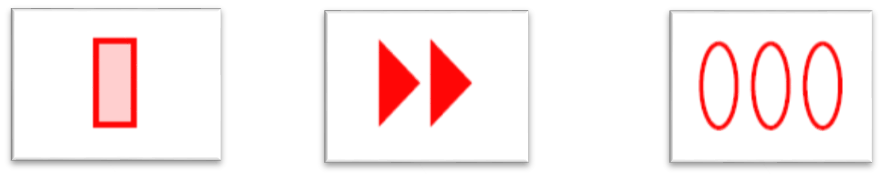
\includegraphics[scale=0.6]{./sachiths_images/image123.png}\\
			\caption[]{\textit{Different types of cards\label{cardtyps}}}
		\end{centering}
	\end{figure}
	
	\begin{figure}[position = here]
		\centering
		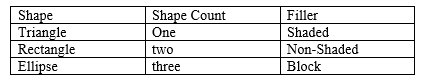
\includegraphics[scale=0.8]{./sachiths_images/image2.png}
		\caption[]{\textit{Variables}}
	\end{figure}

As a part of the system the robot arm was appended with a camera mounted on top of the table which can be used to acquire images of the objects place on the table. These images can be used to identify the object properties using image processing techniques. 

There are plenty of approaches to find features in image processing such as:

\begin{enumerate}
	\item Edge detection
	\item Binary image processing\cite{MachineVision}
	\item Corner detection
	\item Hough transformation
	\item Swift operator
	\item Histogram comparisons
\end{enumerate}

In this project Edge detection and Binary image processing methods were heavily used to identify the cards from the table and shapes in the cards.

\subsubsection{Edge Detection}
An edge in an image is a significant local change in the image intensity, usually associated with a discontinuity in either the image intensity or the first derivative of the image intensity\cite{MachineVision}. The inbuilt Matlab toolbox  for edge detection (the Canny\cite{Canny} operator) was our primary port of call for this project.

\subsubsection{Binary image processing} Using a histogram of the image a threshold can be identified to convert the image to a binary image with areas of interests. This method was feasible to this project as the back of the card gives pixel values that can be approximated to black whereas the front of the card gives pixel values nearer to white, allowing this to be a core factor in differentiating cards that were face up or face down. 

After creating the binary image with interested regions Matlab's inbuilt functions can be used to identify centroids and orientations of the interested regions. Local positions can be transferred to world coordinates using a simple coordinate geometric calculation based on the 3 fiducial boxes placed in position. Fiducials can effectively be anything (including the manipulator arm itself) but it was simpler to use a fiducial that we knew was as close as possible to the table in order to minimise the need to calculcate object depth correlations between the arm in the air and the cards on the table.
